\documentclass[a4paper,11pt]{article}

\usepackage{mlsubmit}
\usepackage{subcaption}


\begin{document}

\initmlsubmision{4} % assignment number
{Piyush Bagad}   % your name
{150487}	% your roll number

\begin{mlsolution}
Let $X$ be the $N\times D$ data matrix. The covariance matrix is given by (assuming centered data) $S = \frac{1}{N}X^{T}X$. Let $T  = \frac{1}{N}XX^{T}$. Suppose $\lambda$ is an eigenvalue and $\vec{v}$ is an eigenvector of $T$, then my claim is that 
$\lambda$ is also an eigenvalue of $S$ with corressponding eigenvector being $X^{T}\vec{v}$. The proof follows:
\[
T\vec{v} = \lambda \vec{v}
\]
\[
\therefore \frac{1}{N}XX^{T}\vec{v} = \lambda \vec{v}
\]
\[
\therefore \frac{1}{N}X^{T}XX^{T}\vec{v} = \lambda X^{T}\vec{v}
\]
\[
\therefore S(X^{T}\vec{v}) = \lambda (X^{T}\vec{v})
\]
Let $\vec{u} := X^{T}\vec{v}$. We have $S\vec{u} = \lambda \vec{u}$. Therefore, $\vec{u}$ turns out to be the eigenvector for $S$ coressponding to the eigenvalue $\lambda$. Thus, if we know eigenvectors of matrix $T$, we can find the eigenvectors of matrix $S$ by simple matrix multiplication which is $O(ND)$. The advantage of using this approach to obtain the eigenvectors is that  we will need to diagonalize the $N\times N$ matrix $T$  instead of the $D\times D$ matrix $S$ for getting eigenvectors. Note that we have been given $N <D$. Thus, it is computationally cheaper to obtain eigenvectors in this manner when $D>N$. Also, note that we can kernelize the matrix $T$ and then conduct eigendecomposition of the kernel matrix enabling us to do non-linear PCA. 


\end{mlsolution}

\begin{mlsolution} 

Given $h(x) = x\sigma(\beta x)$ where $\sigma$ is the usual sigmoid activation function.
\[
h(x) = \frac{x}{1+\exp(-\beta x)}
\]

\subsubsection{Case 1: Linear approximation}
Take $\beta = 0$, we will have 
\[
h(x) = \frac{x}{2} \ \ \ \ [\text{Linear}]
\]

\subsubsection{Case 2: Approximating ReLU}
Take $\beta \rightarrow \infty$, we will have $\exp(-\beta x)\rightarrow \infty$ for all $x<0$ and $\exp(-\beta x)\rightarrow 0$ for $x\geq 0$. Thus, we get
\[
h(x) = 
\begin{cases}
0 & \forall x < 0 \\
x & \forall x \geq 0
\end{cases}
\]
Hence, we can approximate ReLU using given activation function $h(x)$.
\end{mlsolution}

\begin{mlsolution}
We have been given data $\{(\textbf{x}_{n}, y_{n})\}_{n=1}^{N}, \textbf{x}_{n}\in \mathbb{R}^{2}, y_n\in \{0,1\}$. We are given 
\[
z_n \sim \text{multinoulli}(\pi_{1}, \pi_{2},..,\pi_{K})
\]
\[
y_n \sim \text{Bernoulli}(\sigma(w^{T}_{z_n}\textbf{x}_{n}))
\]
We want to estimate $p(y_n =1|\textbf{x}_n)$:
\begin{equation*}
p(y_n =1|\textbf{x}_n) = \sum_{k=1}^{K}p(y_n = 1, z_{n} = k|\textbf{x}_n) \\ 
 = \sum_{k=1}^{K}p(y_n = 1 |  z_{n} = k, \textbf{x}_n)p(z_n = k) \\ 
 = \sum_{k=1}^{K} \sigma(w^{T}_{k}\textbf{x}_{n})\pi_{k}
\end{equation*}
\[
\boxed{p(y_n =1|\textbf{x}_n) = \sum_{k=1}^{K} \sigma(w^{T}_{k}\textbf{x}_{n})\pi_{k}}
\]
We can think of this as a neural network in the following way:
\begin{itemize}
	\item \textbf{Input layer}: $(x_{1}, x_{2},..,x_{D}), \textbf{x}\in \mathbb{R}^{D}$ is the input example.
	\item \textbf{Hidden layer}: We consider a single hidden layer of size K with each hidden node $k$ having output $\sigma(w^{T}_{k}\textbf{x})$. The weight matrix will be $\textbf{W} = [w_{ij}], i \in \{1,2,..,D\}, \ j \in \{1,2.,,K\}$ i.e. $\textbf{W} = [w^{T}_{1} \  w^{T}_{2} \ ... \  w^{T}_{K}]$.
	\item \textbf{Final layer}: The output layer will consist of only a single node whose output will be $p(y = 1 | \textbf{x})$. The weight vector $\textbf{U} = [\pi_{1} \ \pi_{2} \ ... \ \pi_{K}]^{T}$.
\end{itemize}

\end{mlsolution}


\begin{mlsolution}
Consider an $N\times M$ rating matrix $X$, where the rows represents the $N$ users and the columns represent the $M$ items. We are also given some side information: for each user $n$, a feature vector $\textbf{a}_n \in \mathbb{R}^{D_U}$ , and for each item $m$, a feature vector $\textbf{b}_{m} \in \mathbb{R}^{D_I}$. Let $\textbf{u}_n$, $\textbf{v}_{m} \in \mathbb{R}^{K}$ represent the latent factors for user $n$ and item $m$ respectively. Let $\theta_n$ be user bias and $\phi_{m}$ be the popularity of item. We have
\[
p(X_{nm} | \textbf{u}_n, \theta_n, \textbf{v}_{m}, \phi_{m}) = \mathcal{N}(X_{nm}| \theta_n + \phi_{m} + \textbf{u}_{n}^{T}\textbf{v}_{m}, \lambda^{-1} )
\]
\[
p(\textbf{u}_n) = \mathcal{N}(\textbf{u}_n | \textbf{W}_{u}\textbf{a}_{n}, \lambda^{-1}_{u}\textbf{I}_{K})
\]
\[
p(\textbf{v}_m) = \mathcal{N}(\textbf{v}_m | \textbf{W}_{v}\textbf{b}_{m}, \lambda^{-1}_{v}\textbf{I}_{K})
\]
Assume $\Omega = \{(n, m)\}$ to denote the set of indices of the observed entries of $X, \Omega_{r_n}$ to be the set of items rated by user $n$, and $\Omega_{c_m}$ to be the set of users who rated item $m$. Let $\Theta := \{ \{(\textbf{u}_{n}, \theta_n)\}, \{\textbf{v}_{m}, \phi_{m}\}, \textbf{W}_{u}, \textbf{W}_{v} \}$.

The MAP objective can be written as follows:
\[
\hat{\Theta}_{MAP} = \arg \max_{\Theta} \{\log(p(X|\Theta)) + \log(p(\Theta))\}
\]
\[
\log(p(X|\Theta)) = \sum_{(n,m)\in \Omega}\log(p(X_{nm} | \Theta)) = -\frac{\lambda}{2}\sum_{(n,m)\in \Omega}(X_{nm} -(\theta_n + \phi_{m} + \textbf{u}_{n}^{T}\textbf{v}_{m}))^{2}
\]
\[
\log(p(\Theta)) = \sum_{n=1}^{N}\log(p(\textbf{u}_{n})) + \sum_{m=1}^{M}\log(p(\textbf{v}_{m})) =  -\frac{\lambda_{u}}{2}\sum_{n=1}^{N} \lVert \textbf{u}_{n} - \textbf{W}_{u}\textbf{a}_{n} \rVert^{2} -\frac{\lambda_{v}}{2}\sum_{m=1}^{M} \lVert \textbf{v}_{m} - \textbf{W}_{v}\textbf{b}_{m} \rVert^{2}
\]
Thus, the consolidated loss can be written as 
\[
\mathcal{L}(\Theta) = \frac{\lambda}{2}\sum_{(n,m)\in \Omega}(X_{nm} - (\theta_n + \phi_{m} + \textbf{u}_{n}^{T}\textbf{v}_{m}))^{2} + \frac{\lambda_{u}}{2}\sum_{n=1}^{N} \lVert \textbf{u}_{n} - \textbf{W}_{u}\textbf{a}_{n} \rVert^{2} +\frac{\lambda_{v}}{2}\sum_{m=1}^{M} \lVert \textbf{v}_{m} - \textbf{W}_{v}\textbf{b}_{m} \rVert^{2}
\]
\subsection{Optimizing using ALT-OPT}
\begin{itemize}
	\item \textbf{Estimating latent variables and parameters for users}: Let us keep $\{\{\hat{\textbf{v}}_{m}, \hat{\phi}_{m}\}, \hat{\textbf{W}}_{v}\}$ fixed and estimate the remaining variables. We will only consider relevant terms in the loss function.
	\[
	\mathcal{L}(\Theta) = \frac{\lambda}{2}\sum_{(n,m)\in \Omega}(X_{nm} - (\theta_n + \phi_{m} + \textbf{u}_{n}^{T}\textbf{v}_{m}))^{2} + \frac{\lambda_{u}}{2}\sum_{n=1}^{N} \lVert \textbf{u}_{n} - \textbf{W}_{u}\textbf{a}_{n} \rVert^{2}
	\]
	\begin{enumerate}
		\item Estimating $\textbf{u}_{n}$ keeping $\theta_n , \textbf{W}_{u}$ fixed: Note that this will turn out to be simple a least-squares problem with the prior on $\textbf{u}_{n}$ being non-zero mean. Thus, we can write the solution in closed form as follows:
		\[
		\textbf{u}_{n} = \left( \sum_{m\in \Omega_{r_n}} \textbf{v}^{T}_{m}\textbf{v}_{m} + \lambda_{u}\textbf{I}_{K} \right)^{-1}\left( \lambda_{u}\textbf{W}_{u}\textbf{a}_{n} + \lambda \sum_{m\in \Omega_{r_n}} (X_{nm} - \theta_n - \phi_{m})\textbf{v}_{m} \right)  
		\]
		\item Estimating $\theta_n$ keeping $\textbf{u}_{n}, \textbf{W}_{u}$ fixed: Now, we can simply set the derivative to 0 and obtain $\theta_n$ as follows:
		\[
		\theta_n = \frac{\sum_{m\in \Omega_{r_n}}(X_{nm} - \phi_{m} - \textbf{u}^{T}_{n}\textbf{v}_{m})}{\sum_{m\in \Omega_{r_n}}1}
		\]
		\item  Estimating $\textbf{W}_{u}$ keeping $\theta_{n}, \textbf{u}_{n}, \forall n $ fixed: This time we get the loss function which resembles the loss of a multi-output linear regression problem. Thus, we can write the solution as follows -
		\[
		\textbf{W}_{u} = \left( \sum_{n=1}^{N}\textbf{u}_{n}\textbf{a}^{T}_{n} \right) \left( \sum_{n=1}^{N}\textbf{a}_{n}\textbf{a}^{T}_{n}\right)^{-1}
		\]
	\end{enumerate}
	\item \textbf{Estimating latent variables and parameters for items}: Similar procedure (as for estiminating user variables and paramters) can be followed for items.
	\begin{enumerate}
		\item Estimating $\textbf{v}_{m}$ keeping $\phi_m , \textbf{W}_{v}$ fixed: 
		\[
		\textbf{v}_{m} = \left( \sum_{n\in \Omega_{c_m}} \textbf{u}^{T}_{n}\textbf{u}_{n} + \lambda_{v}\textbf{I}_{K} \right)^{-1}\left( \lambda_{v}\textbf{W}_{v}\textbf{b}_{m} + \lambda \sum_{n\in \Omega_{c_m}} (X_{nm} - \theta_n - \phi_{m})\textbf{u}_{n} \right)  
		\]
		\item Estimating $\phi_m$ keeping $\textbf{v}_{m}, \textbf{W}_{v}$ fixed:
		\[
		\phi_m = \frac{\sum_{n\in \Omega_{c_m}}(X_{nm} - \theta_{n} - \textbf{u}^{T}_{n}\textbf{v}_{m})}{\sum_{n\in \Omega_{c_m}}1}
		\]
		\item  Estimating $\textbf{W}_{v}$ keeping $\phi_{m}, \textbf{v}_{m}, \forall m $ fixed:
		\[
		\textbf{W}_{v} = \left( \sum_{m=1}^{M}\textbf{v}_{m}\textbf{b}^{T}_{m} \right) \left( \sum_{m=1}^{M}\textbf{b}_{m}\textbf{b}^{T}_{m}\right)^{-1}
		\]
	\end{enumerate}
\end{itemize}

\end{mlsolution}

\begin{mlsolution}

% My solution to problem 6
\subsection{Part 1: PPCA using ALT-OPT}
The follwoing section shows visual results for the PPCA task for each of the values of $K \in \{10,20,30,40,50,100\}$. I observed that the image quality certainly improves on increasing K. As evident from the results for $K = 100$, it almost exactly reproduces the original images. Also, I observed that on further increasing $K$, the quality dropped down possibly due to overfitting. Appropriate regularization helped in avoiding overfitting. For each K, I have also shown the first 10 columns of matrix $W$. It resembles the templates of images which the model will be using to reconstruct original images as a linear combination. For K =10, it seems that $W$ has a very rough structure which does not focus on the minor details of the faces but only focusses on the high-level characteristics. Whereas for higher K, the details included in the template images seem to increase. It seems that for higher K, each of the columns of W is a better template to reconstruct many original images. In other words, each column of W is formed from knowledge about multiple original images.
\begin{figure}[!htbp]
	\centering
	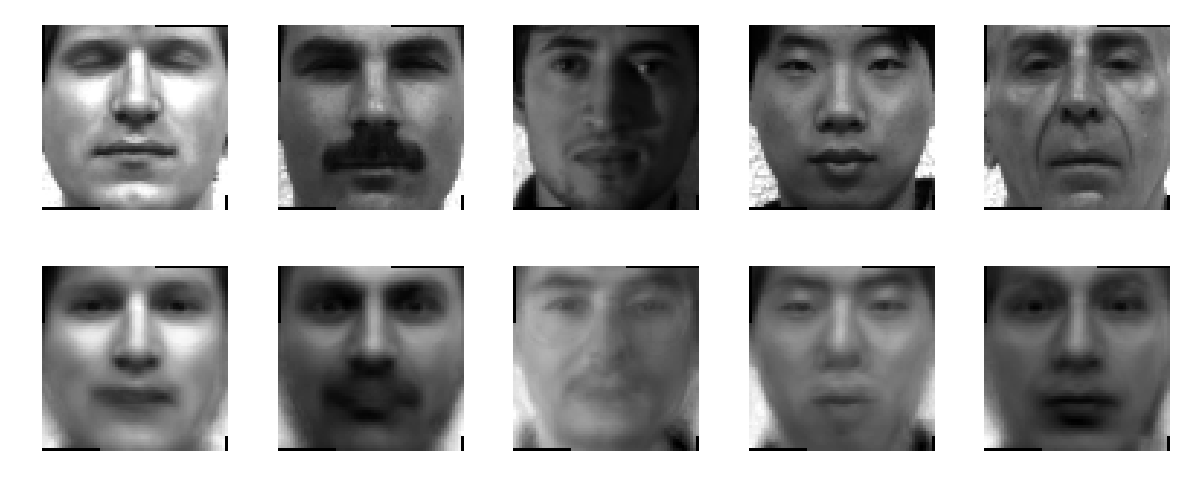
\includegraphics[width=0.9\textwidth, height=0.4\linewidth]{images/img_k_10.png}
	\caption[k = 10]{Reconstructed images of randomly chosen samples for K = 10.}
\end{figure}
\begin{figure}[!htbp]
	\centering
	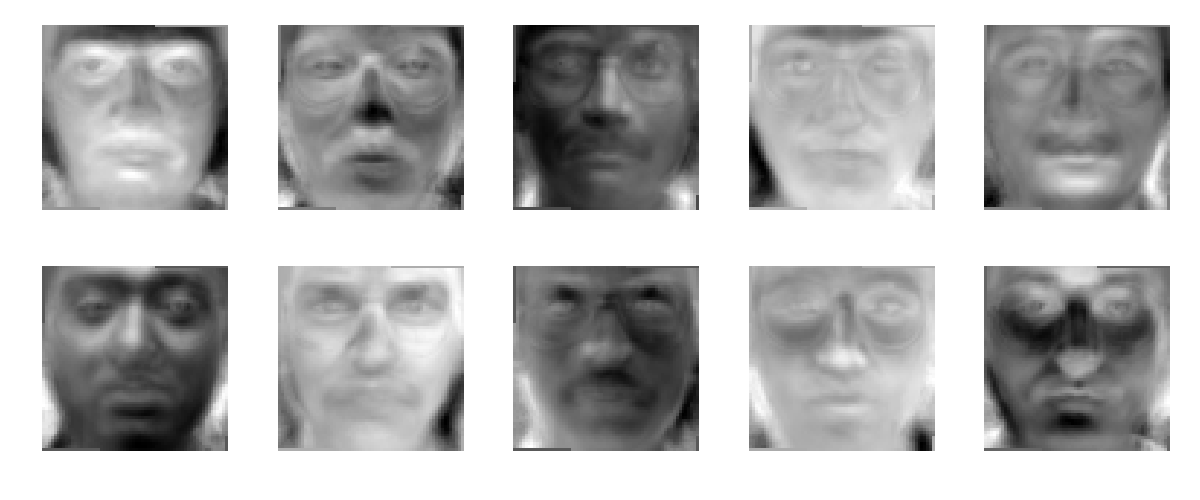
\includegraphics[width=0.9\textwidth, height=0.4\linewidth]{images/template_weights_k_10.png}
	\caption[k = 10]{Basis images for K = 10.}
\end{figure}


\begin{figure}[!htbp]
	\centering
	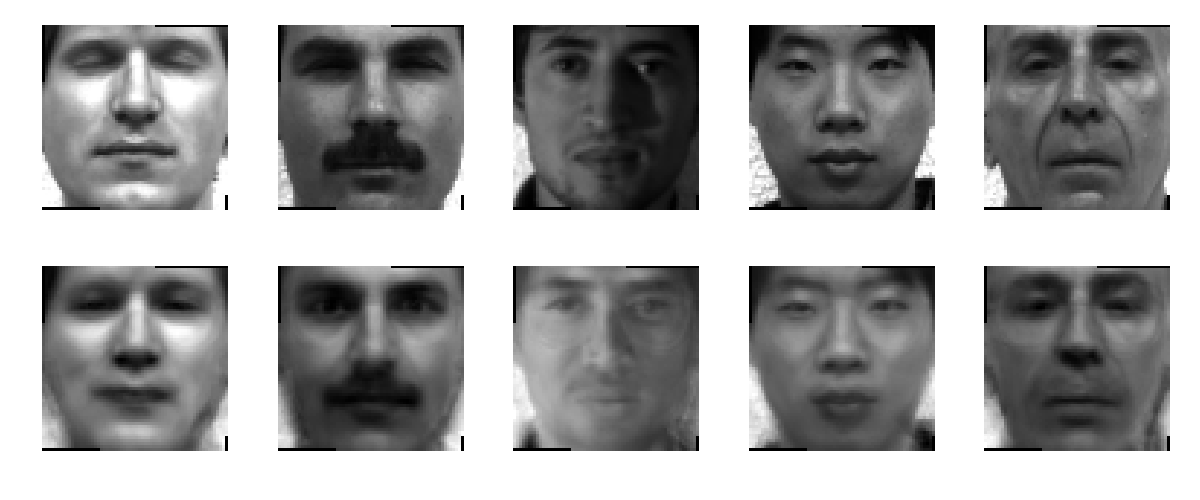
\includegraphics[width=0.9\textwidth, height=0.4\linewidth]{images/img_k_20.png}
	\caption[k = 20]{Reconstructed images of randomly chosen samples for K = 20.}
\end{figure}
\begin{figure}[!htbp]
	\centering
	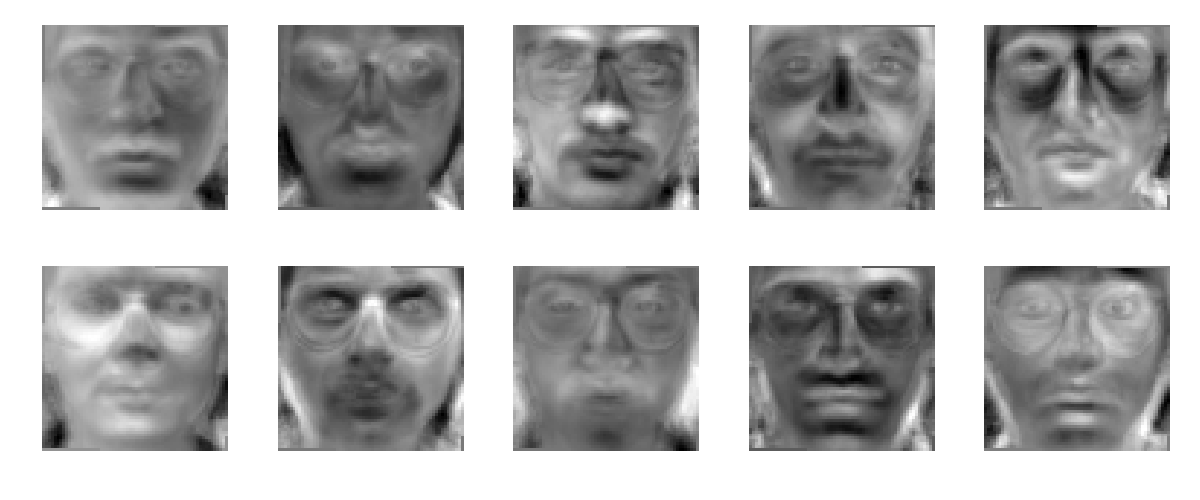
\includegraphics[width=0.9\textwidth, height=0.4\linewidth]{images/template_weights_k_20.png}
	\caption[k = 20]{Basis images for K = 20.}
\end{figure}

\begin{figure}[!htbp]
	\centering
	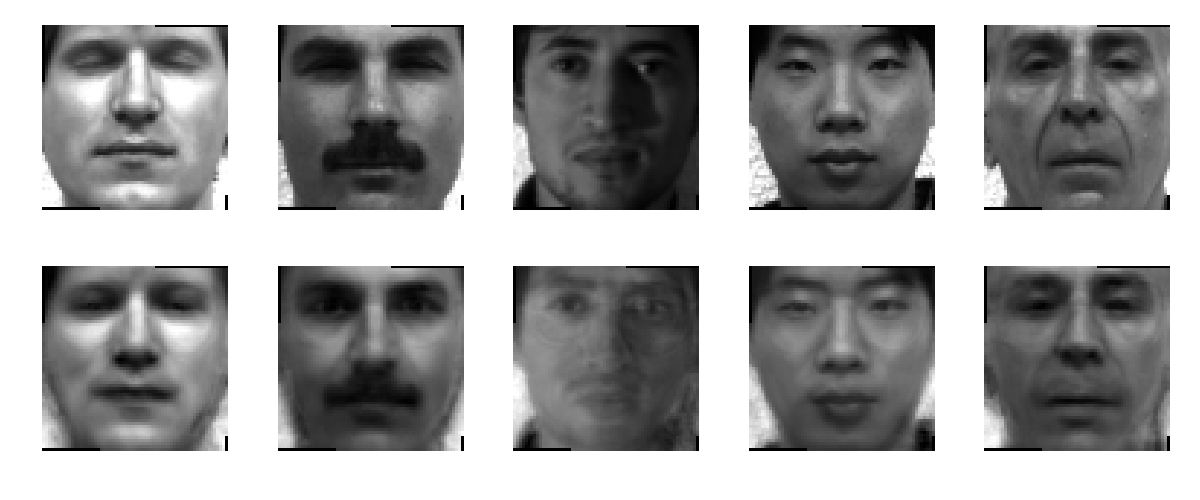
\includegraphics[width=0.9\textwidth, height=0.4\linewidth]{images/img_k_30.png}
	\caption[k = 30]{Reconstructed images of randomly chosen samples for K = 30.}
\end{figure}
\begin{figure}[!htbp]
	\centering
	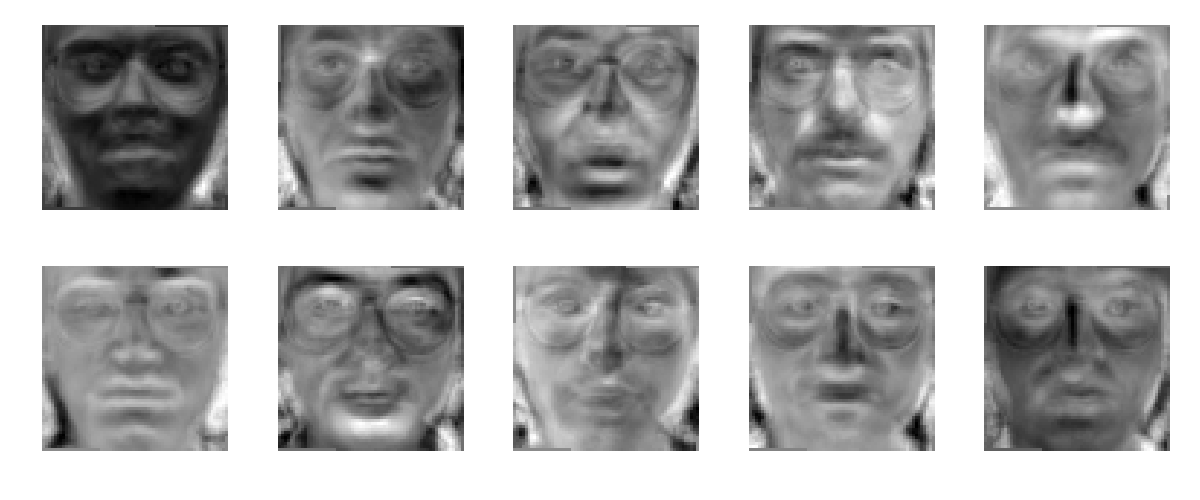
\includegraphics[width=0.9\textwidth, height=0.4\linewidth]{images/template_weights_k_30.png}
	\caption[k = 30]{Basis images for K = 30.}
\end{figure}

\begin{figure}[!htbp]
	\centering
	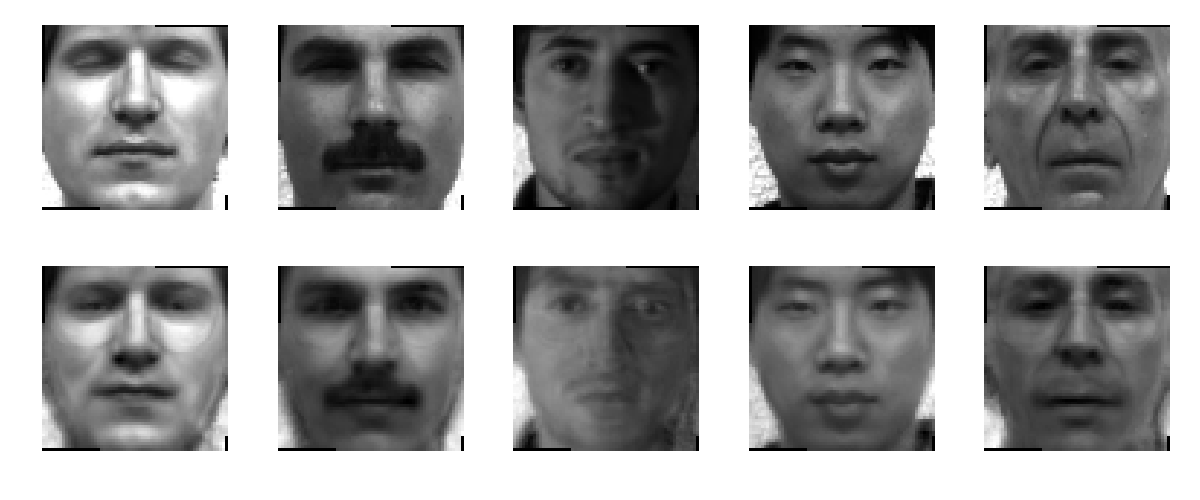
\includegraphics[width=0.9\textwidth, height=0.4\linewidth]{images/img_k_40.png}
	\caption[k = 40]{Reconstructed images of randomly chosen samples for K = 40.}
\end{figure}
\begin{figure}[!htbp]
	\centering
	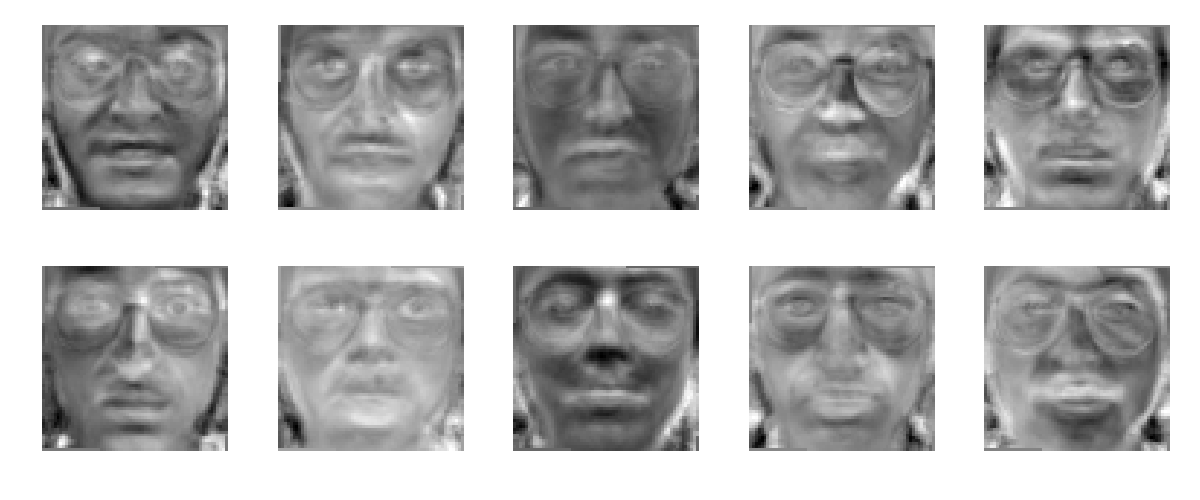
\includegraphics[width=0.9\textwidth, height=0.4\linewidth]{images/template_weights_k_40.png}
	\caption[k = 40]{Basis images for K = 40.}
\end{figure}

\begin{figure}[!htbp]
	\centering
	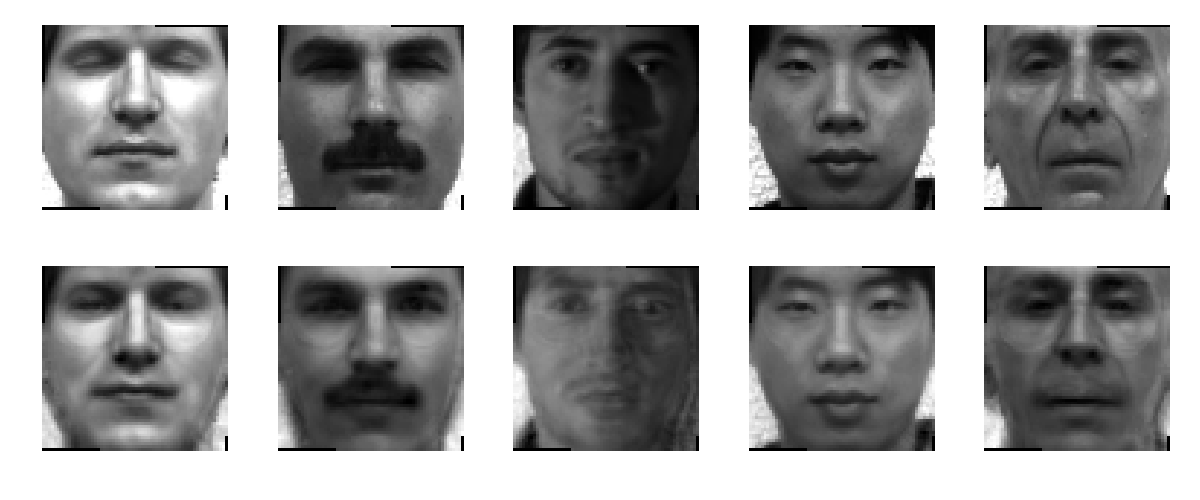
\includegraphics[width=0.9\textwidth, height=0.4\linewidth]{images/img_k_50.png}
	\caption[k = 50]{Reconstructed images of randomly chosen samples for K = 50.}
\end{figure}
\begin{figure}[!htbp]
	\centering
	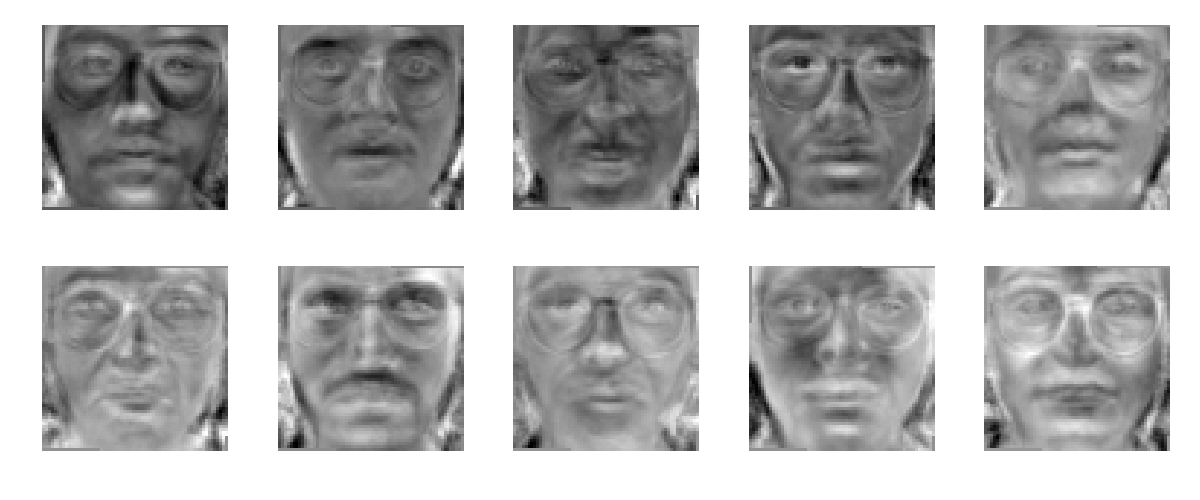
\includegraphics[width=0.9\textwidth, height=0.4\linewidth]{images/template_weights_k_50.png}
	\caption[k = 50]{Basis images for K = 50.}
\end{figure}

\begin{figure}[!htbp]
	\centering
	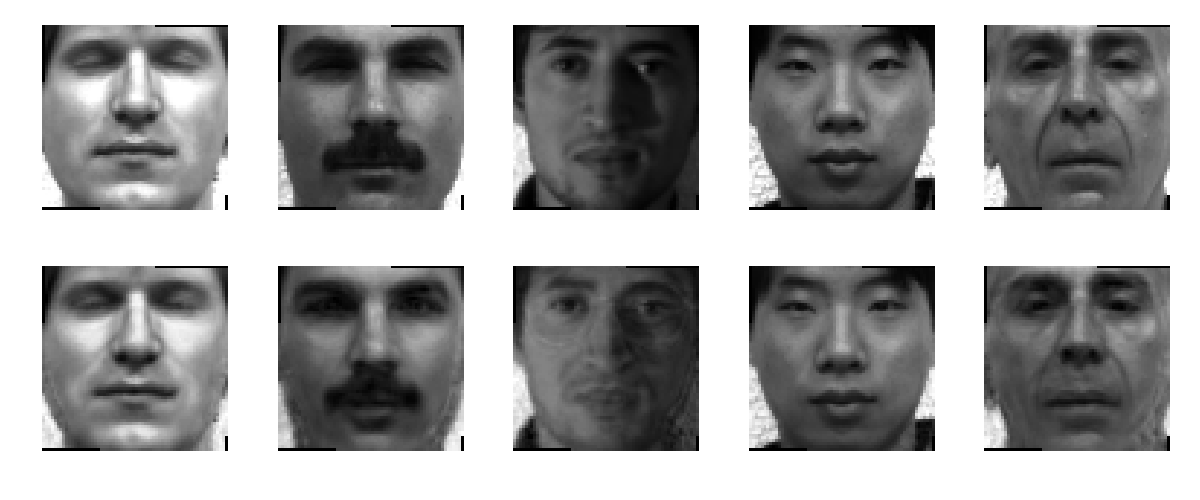
\includegraphics[width=0.9\textwidth, height=0.4\linewidth]{images/img_k_100.png}
	\caption[k = 100]{Reconstructed images of randomly chosen samples for K = 100.}
\end{figure}
\begin{figure}[!htbp]
	\centering
	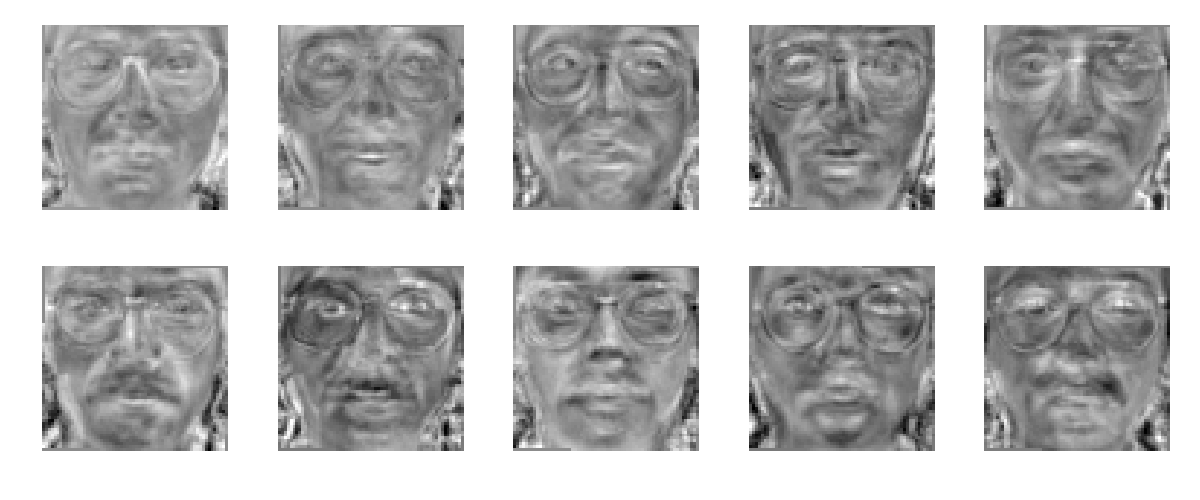
\includegraphics[width=0.9\textwidth, height=0.4\linewidth]{images/template_weights_k_100.png}
	\caption[k = 100]{Basis images for K = 100.}
\end{figure}

\pagebreak

\subsection{Part 2: kMeans Clustering}
This section shows clustering results on the 2D embeddings produced by either PCA or TSNE. The clustering seem to be better for tSNE primarily because:
\begin{itemize}
	\item It focusses more on pair wise distances and tries to preserve local structure. Here, say for instance, all images coressponding to 0 will look similar as against those for 1 or tohers. Thus, even in the embedding space they must be closer. This is evident from the plots.
	\item kMeans assumes approximately similar cluster sizes and shapes. However, PCA since it does not focus on local neighborhoods given sort of a homogenous embedded dataset with hardly any distinctions across classes.
\end{itemize}


\subsubsection{A] With PCA: 10 random initializations}

\begin{figure}[!htbp]
	\begin{subfigure}{.5\textwidth}
		\centering
		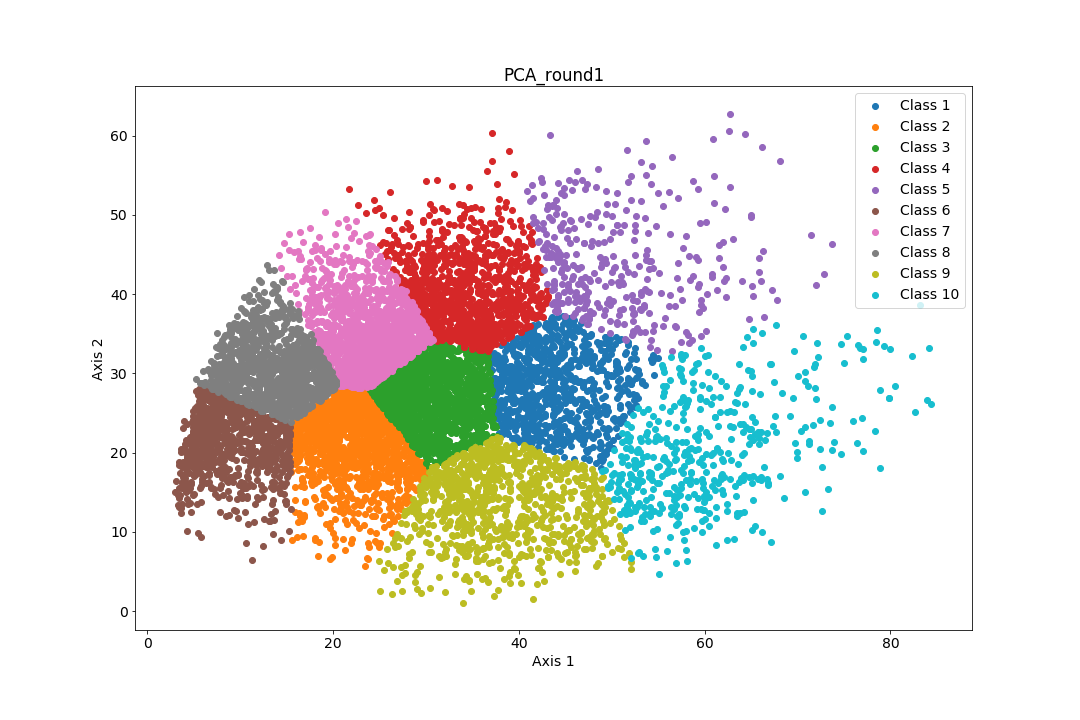
\includegraphics[width=1.1\linewidth]{PCA_round1_kMeans.png}
		\caption{Clustering with PCA: Round 1}
		\label{pca1}
	\end{subfigure}%
	\begin{subfigure}{.5\textwidth}
		\centering
		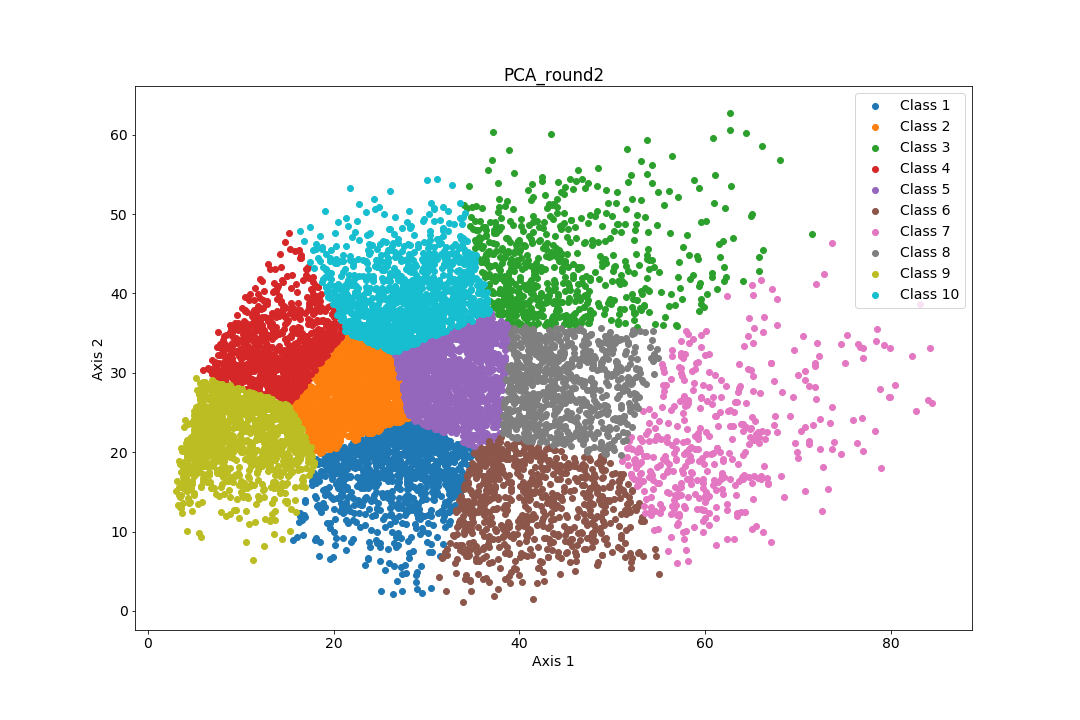
\includegraphics[width=1.1\linewidth]{PCA_round2_kMeans.png}
		\caption{Clustering with PCA: Round 2}
		\label{pca2}
	\end{subfigure}
\end{figure}

\begin{figure}[!htbp]
	\begin{subfigure}{.5\textwidth}
		\centering
		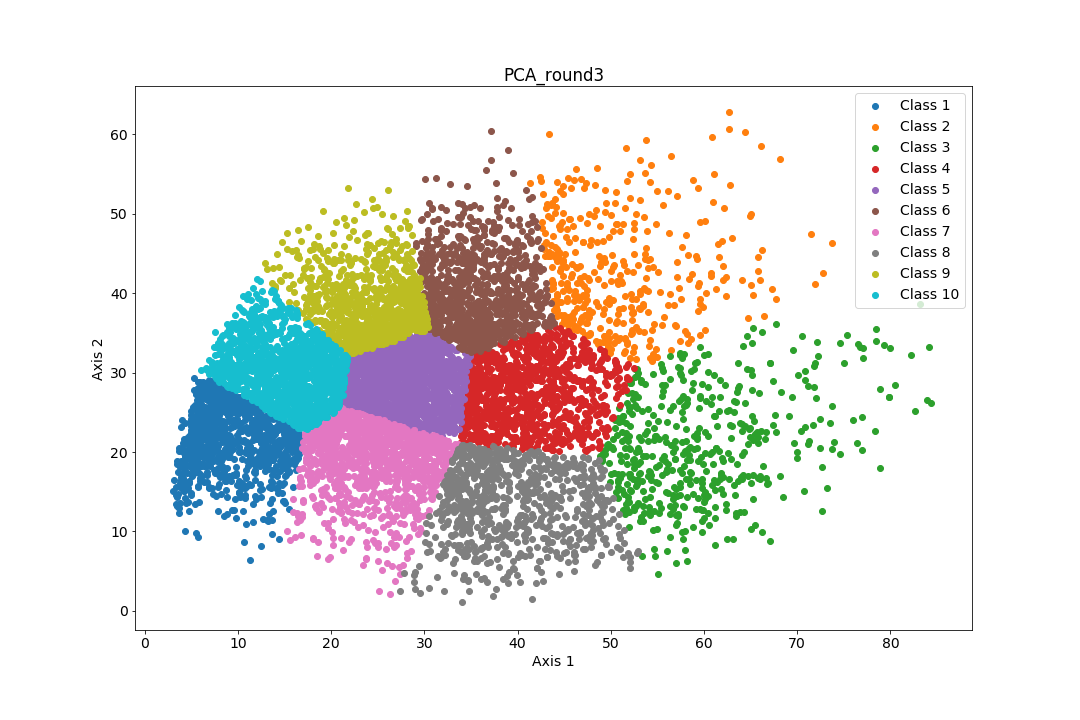
\includegraphics[width=1.1\linewidth]{PCA_round3_kMeans.png}
		\caption{Clustering with PCA: Round 3}
		\label{pca3}
	\end{subfigure}%
	\begin{subfigure}{.5\textwidth}
		\centering
		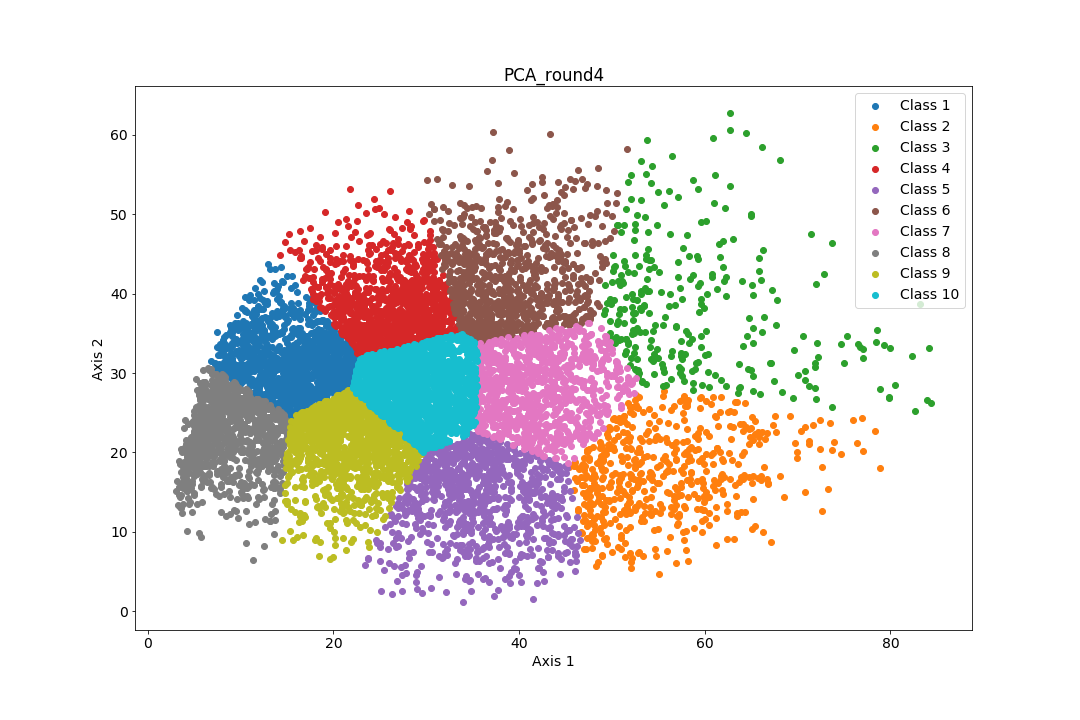
\includegraphics[width=1.1\linewidth]{PCA_round4_kMeans.png}
		\caption{Clustering with PCA: Round 4}
		\label{pca4}
	\end{subfigure}
\end{figure}

\begin{figure}[!htbp]
	\begin{subfigure}{.5\textwidth}
		\centering
		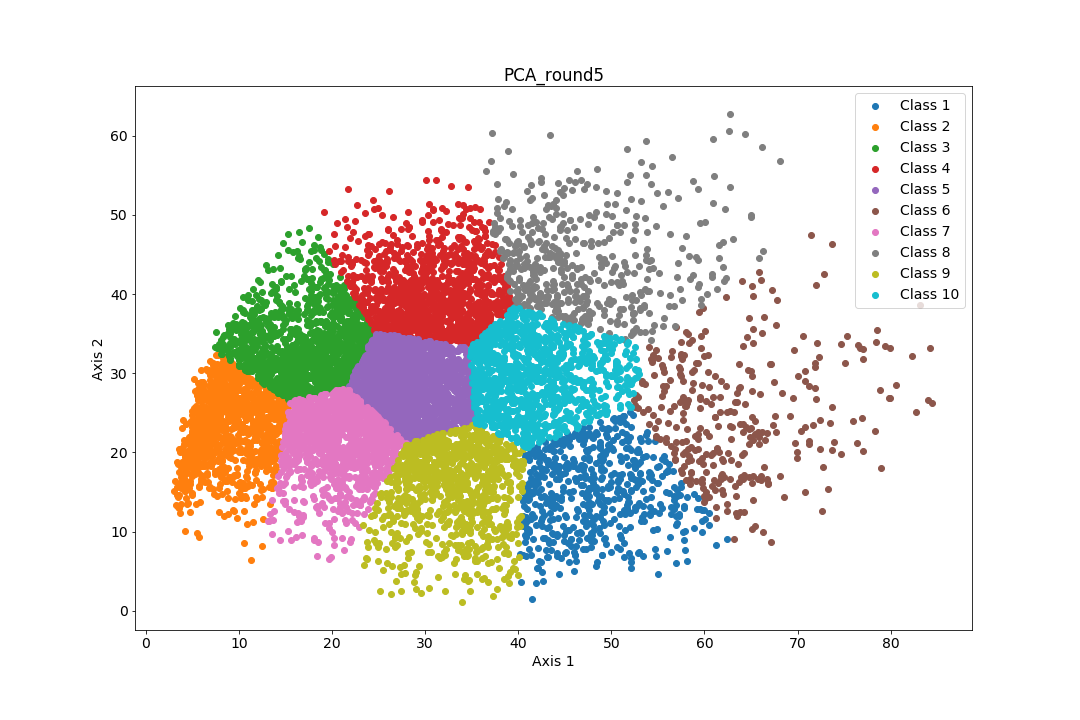
\includegraphics[width=1.1\linewidth]{PCA_round5_kMeans.png}
		\caption{Clustering with PCA: Round 5}
		\label{pca5}
	\end{subfigure}%
	\begin{subfigure}{.5\textwidth}
		\centering
		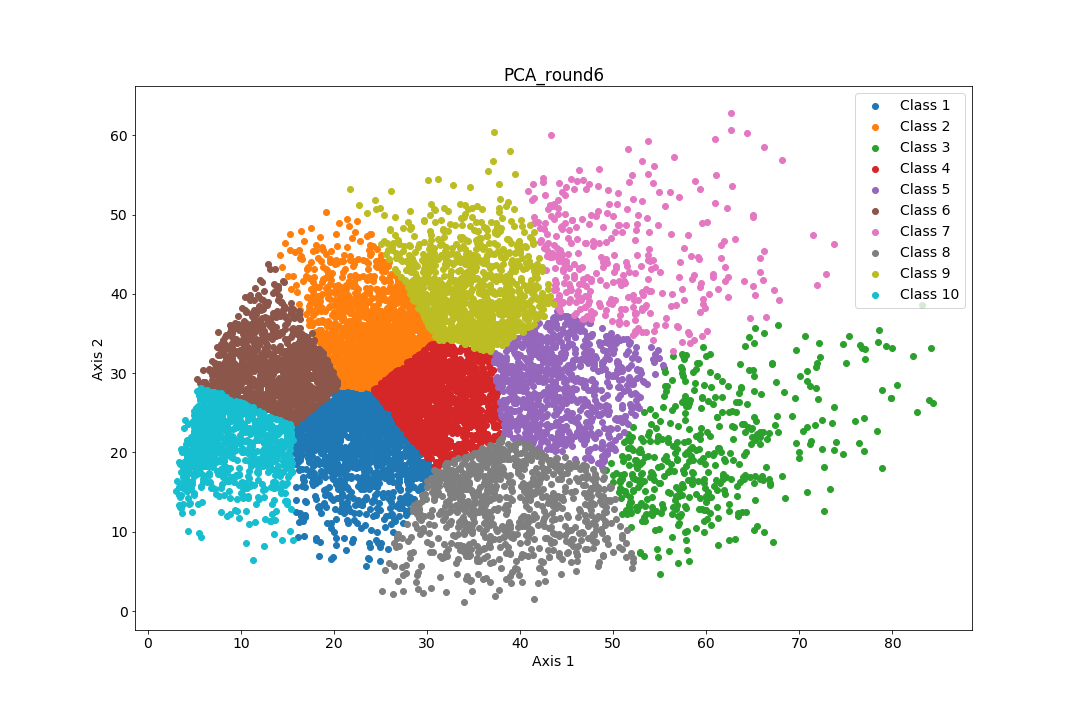
\includegraphics[width=1.1\linewidth]{PCA_round6_kMeans.png}
		\caption{Clustering with PCA: Round 6}
		\label{pca6}
	\end{subfigure}
\end{figure}

\begin{figure}[!htbp]
	\begin{subfigure}{.5\textwidth}
		\centering
		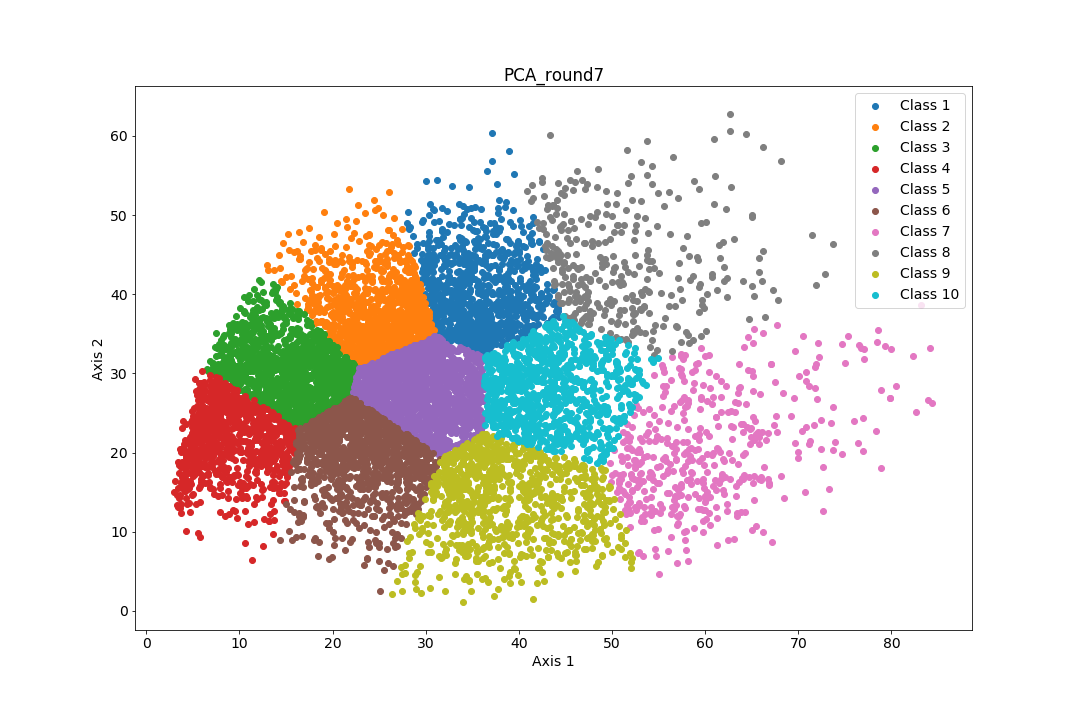
\includegraphics[width=1.1\linewidth]{PCA_round7_kMeans.png}
		\caption{Clustering with PCA: Round 7}
		\label{pca7}
	\end{subfigure}%
	\begin{subfigure}{.5\textwidth}
		\centering
		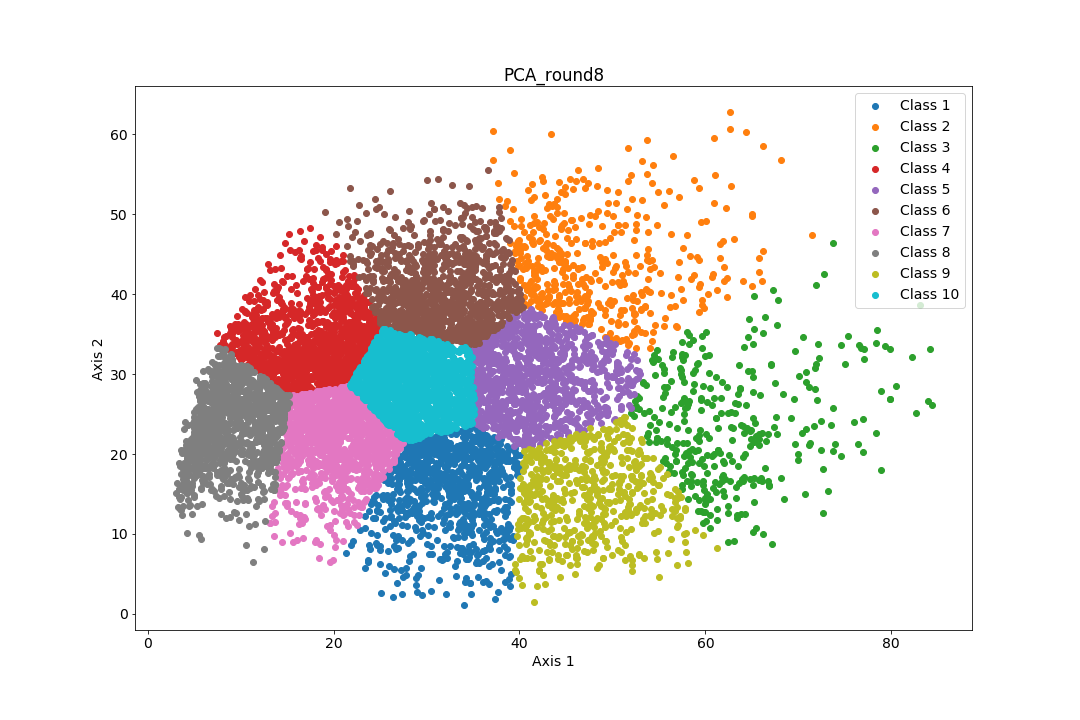
\includegraphics[width=1.1\linewidth]{PCA_round8_kMeans.png}
		\caption{Clustering with PCA: Round 8}
		\label{pca8}
	\end{subfigure}
\end{figure}

\begin{figure}[!htbp]
	\begin{subfigure}{.5\textwidth}
		\centering
		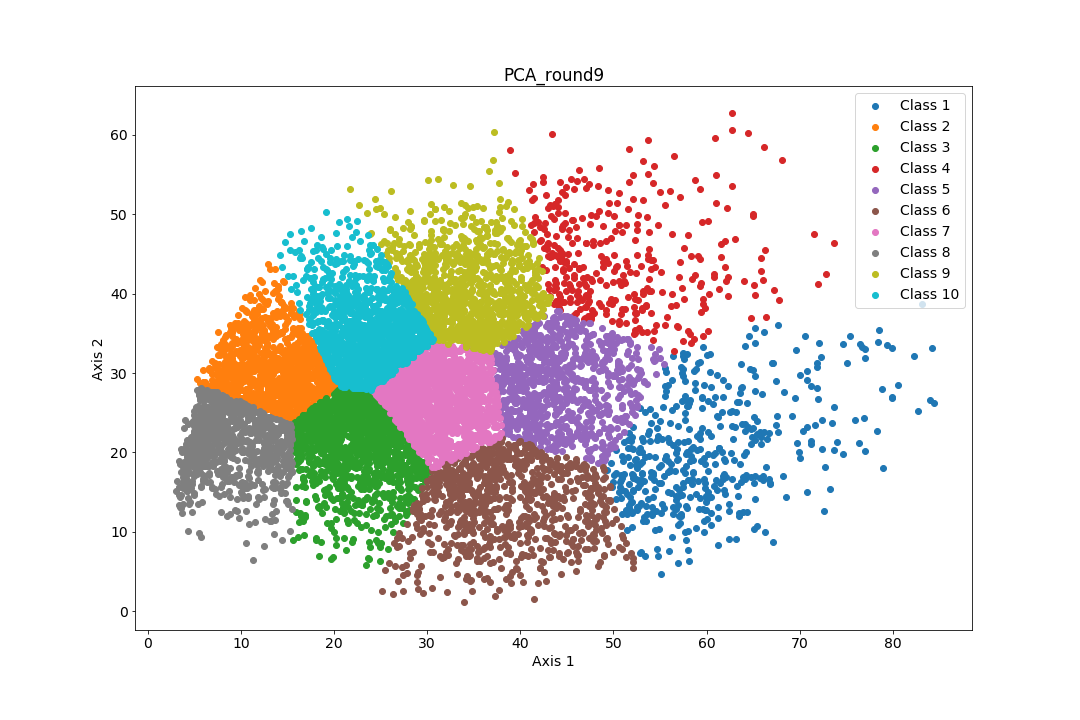
\includegraphics[width=1.1\linewidth]{PCA_round9_kMeans.png}
		\caption{Clustering with PCA: Round 9}
		\label{pca9}
	\end{subfigure}%
	\begin{subfigure}{.5\textwidth}
		\centering
		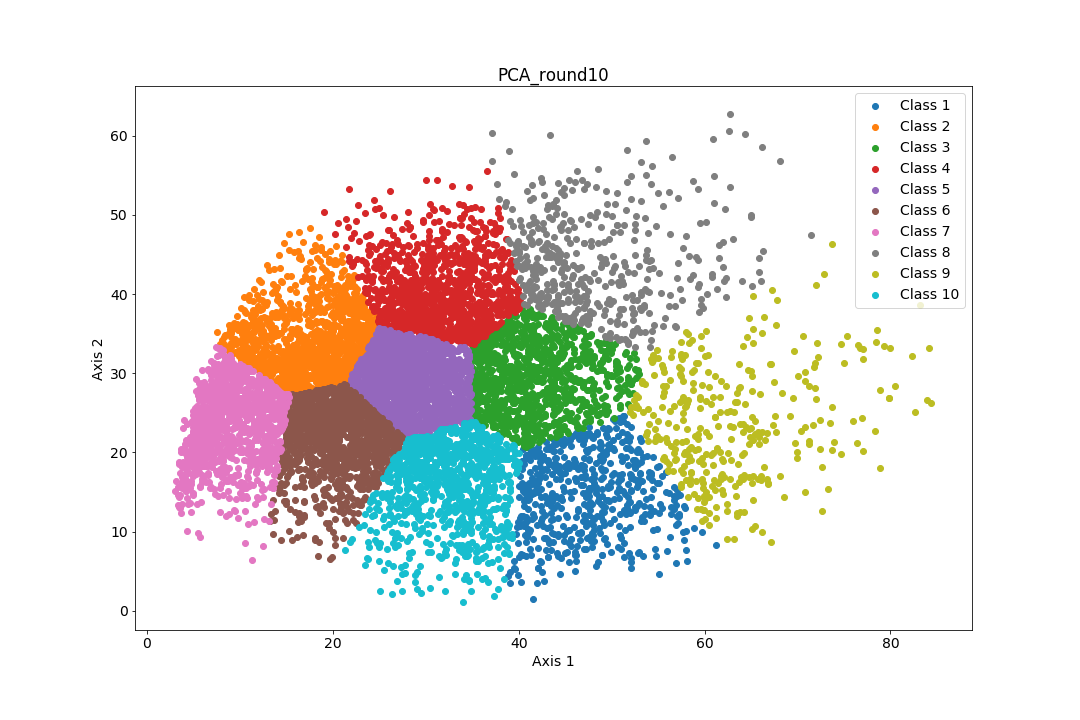
\includegraphics[width=1.1\linewidth]{PCA_round10_kMeans.png}
		\caption{Clustering with PCA: Round 10}
		\label{pca10}
	\end{subfigure}
\end{figure}

\pagebreak

\subsubsection{B] With t-SNE: 10 random initializations}

\begin{figure}[!htbp]
	\begin{subfigure}{.5\textwidth}
		\centering
		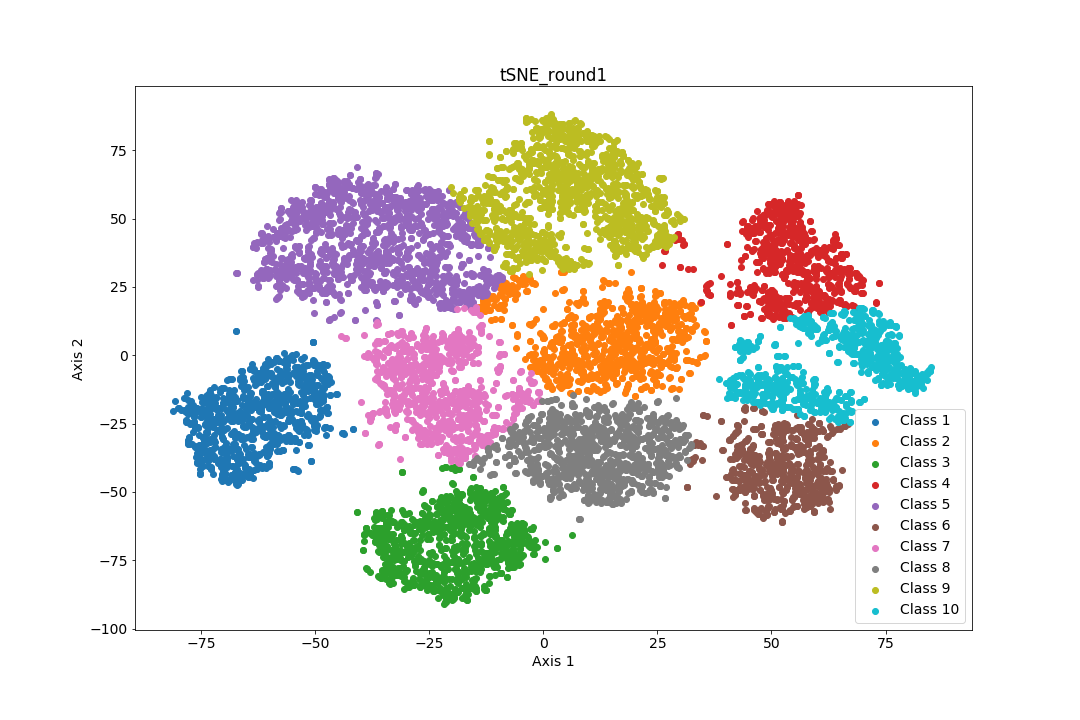
\includegraphics[width=1.1\linewidth]{tSNE_round1_kMeans.png}
		\caption{Clustering with tSNE: Round 1}
		\label{tSNE1}
	\end{subfigure}%
	\begin{subfigure}{.5\textwidth}
		\centering
		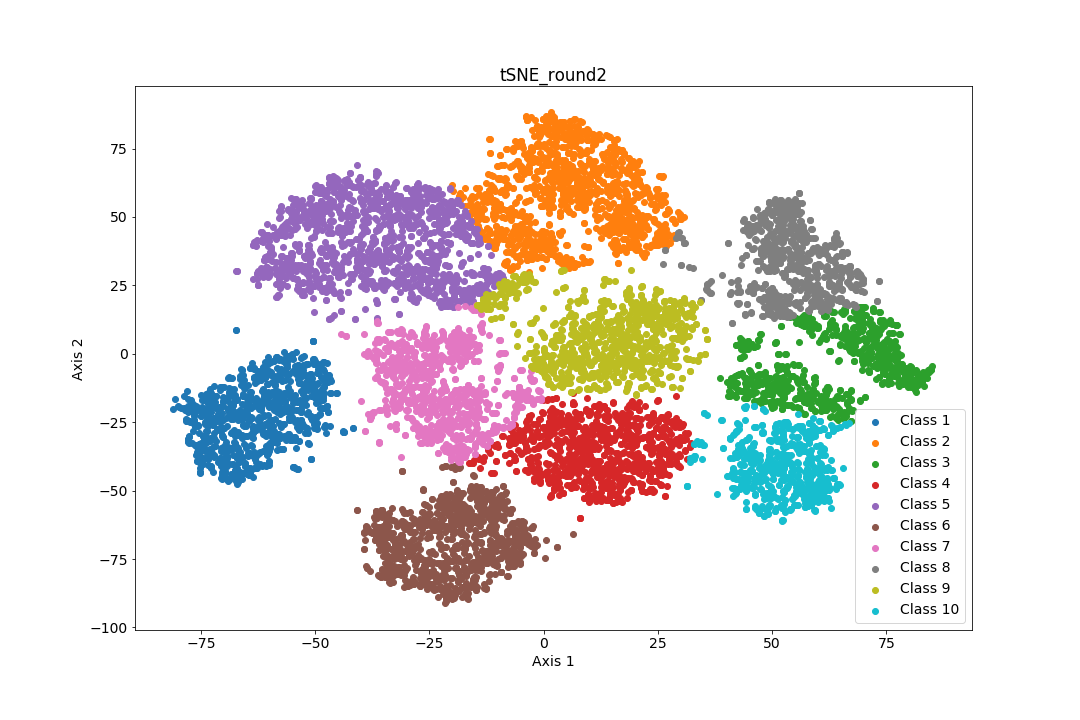
\includegraphics[width=1.1\linewidth]{tSNE_round2_kMeans.png}
		\caption{Clustering with tSNE: Round 2}
		\label{tSNE2}
	\end{subfigure}
\end{figure}

\begin{figure}[!htbp]
	\begin{subfigure}{.5\textwidth}
		\centering
		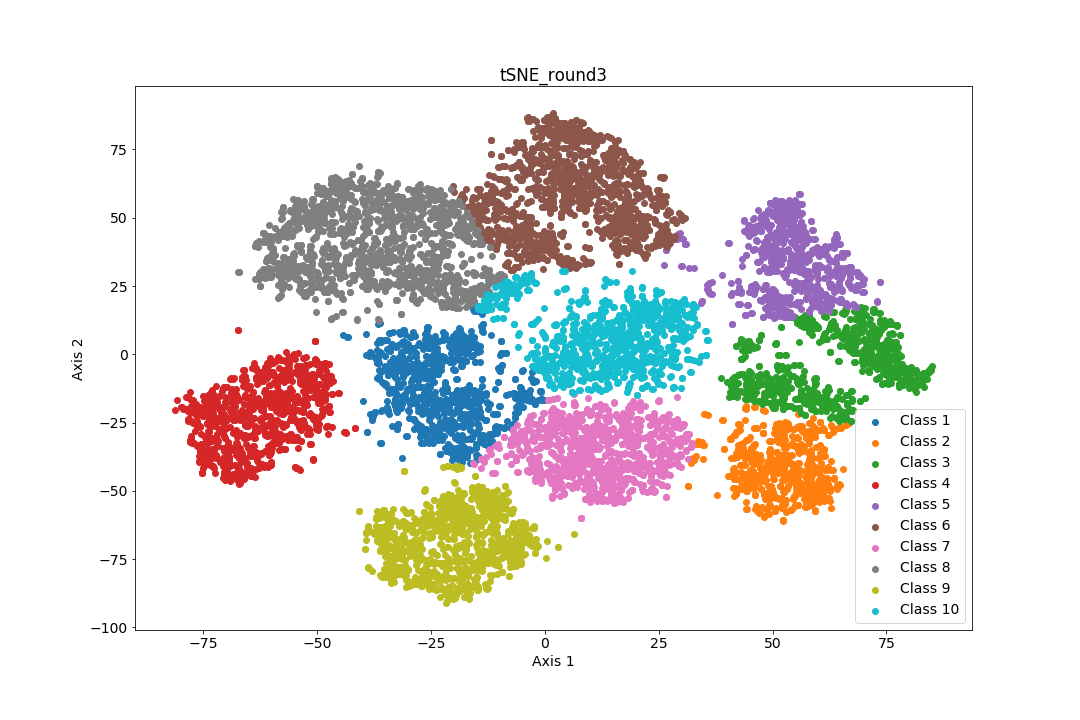
\includegraphics[width=1.1\linewidth]{tSNE_round3_kMeans.png}
		\caption{Clustering with tSNE: Round 3}
		\label{tSNE3}
	\end{subfigure}%
	\begin{subfigure}{.5\textwidth}
		\centering
		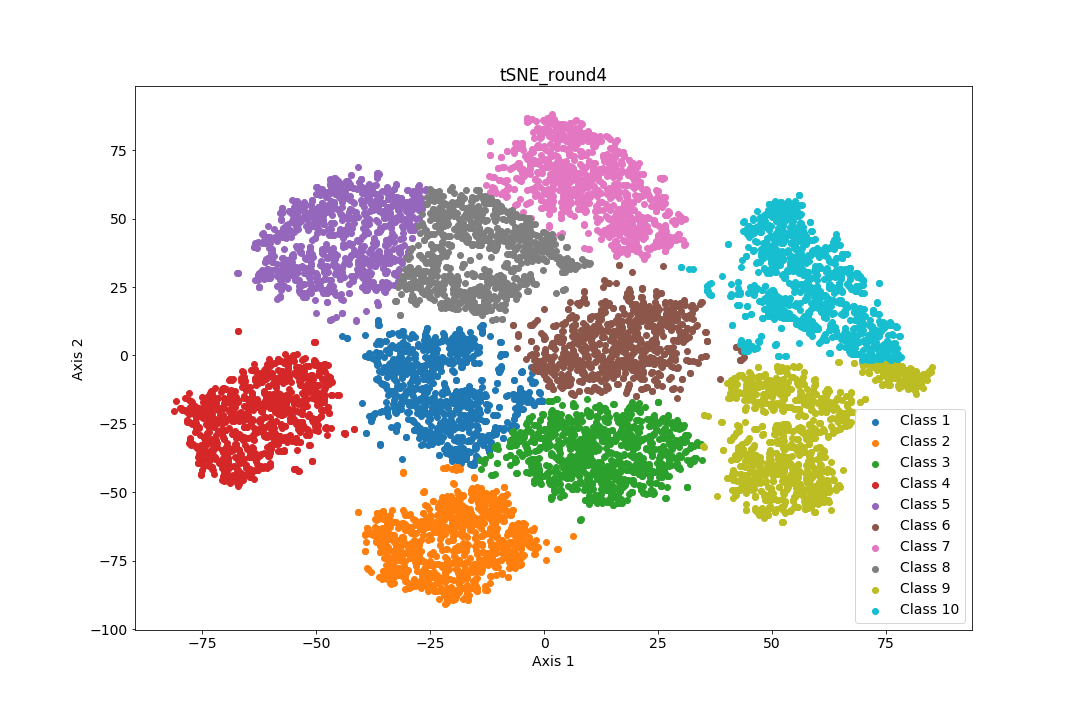
\includegraphics[width=1.1\linewidth]{tSNE_round4_kMeans.png}
		\caption{Clustering with tSNE: Round 4}
		\label{tSNE4}
	\end{subfigure}
\end{figure}

\begin{figure}[!htbp]
	\begin{subfigure}{.5\textwidth}
		\centering
		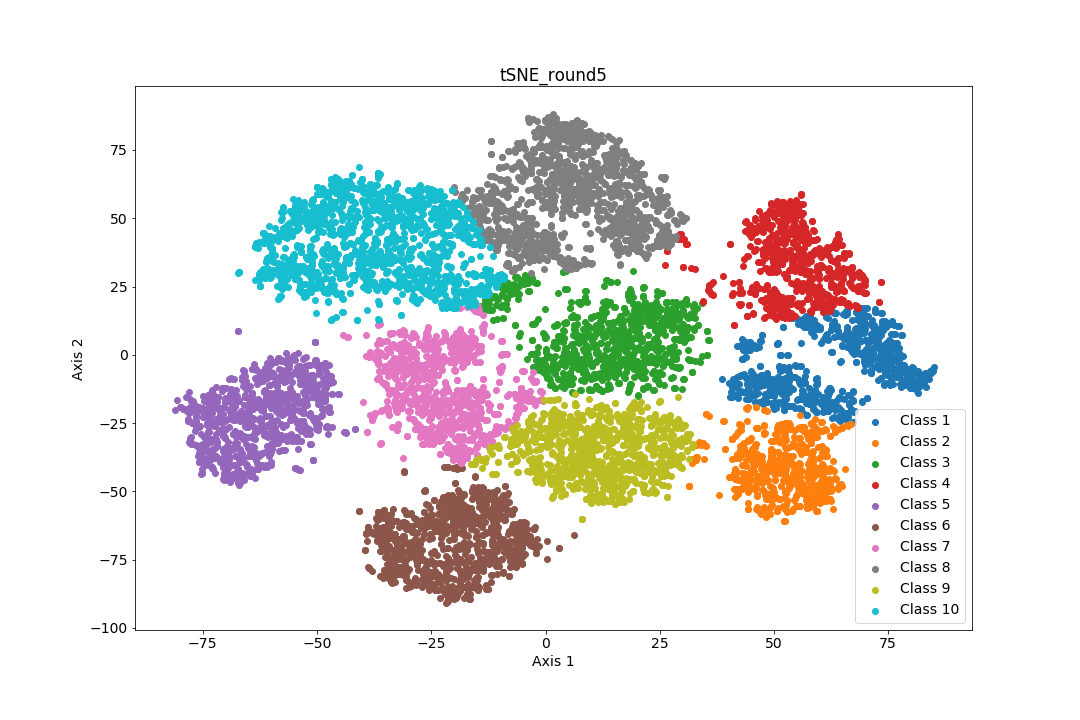
\includegraphics[width=1.1\linewidth]{tSNE_round5_kMeans.png}
		\caption{Clustering with tSNE: Round 5}
		\label{tSNE5}
	\end{subfigure}%
	\begin{subfigure}{.5\textwidth}
		\centering
		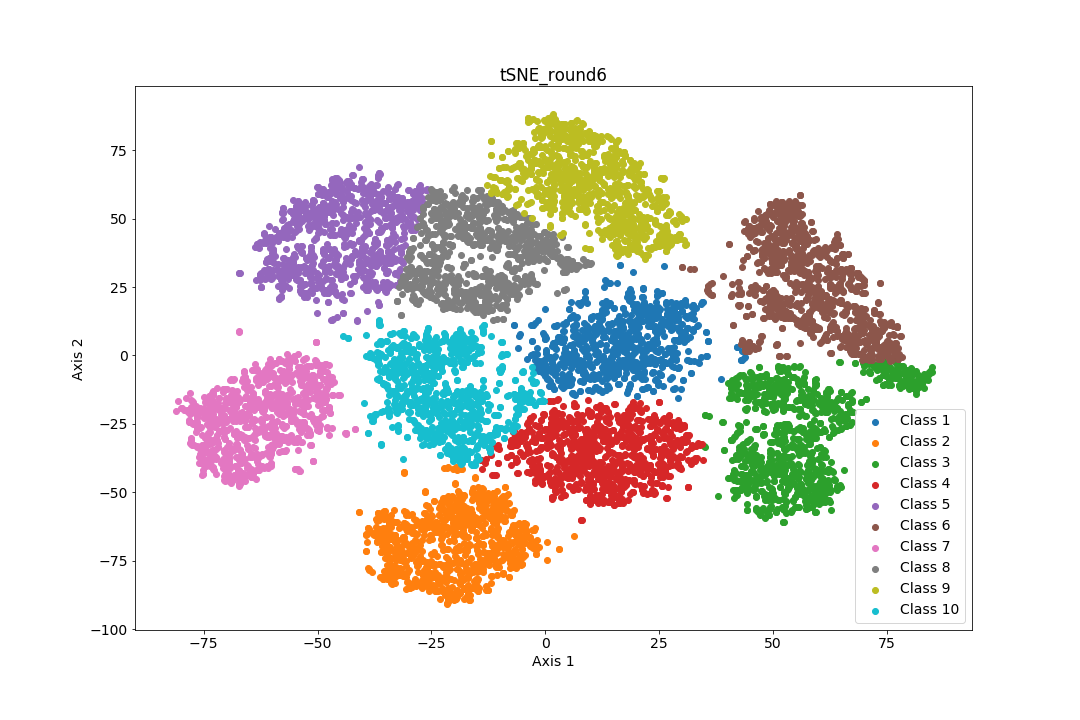
\includegraphics[width=1.1\linewidth]{tSNE_round6_kMeans.png}
		\caption{Clustering with tSNE: Round 6}
		\label{tSNE6}
	\end{subfigure}
\end{figure}

\begin{figure}[!htbp]
	\begin{subfigure}{.5\textwidth}
		\centering
		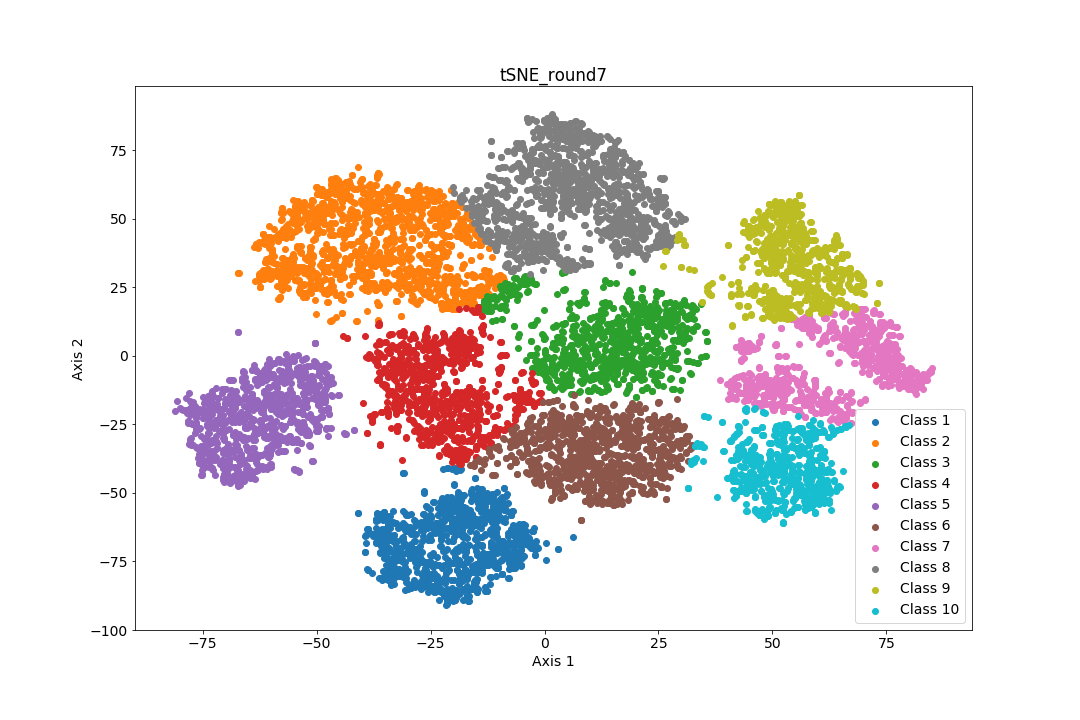
\includegraphics[width=1.1\linewidth]{tSNE_round7_kMeans.png}
		\caption{Clustering with tSNE: Round 7}
		\label{tSNE7}
	\end{subfigure}%
	\begin{subfigure}{.5\textwidth}
		\centering
		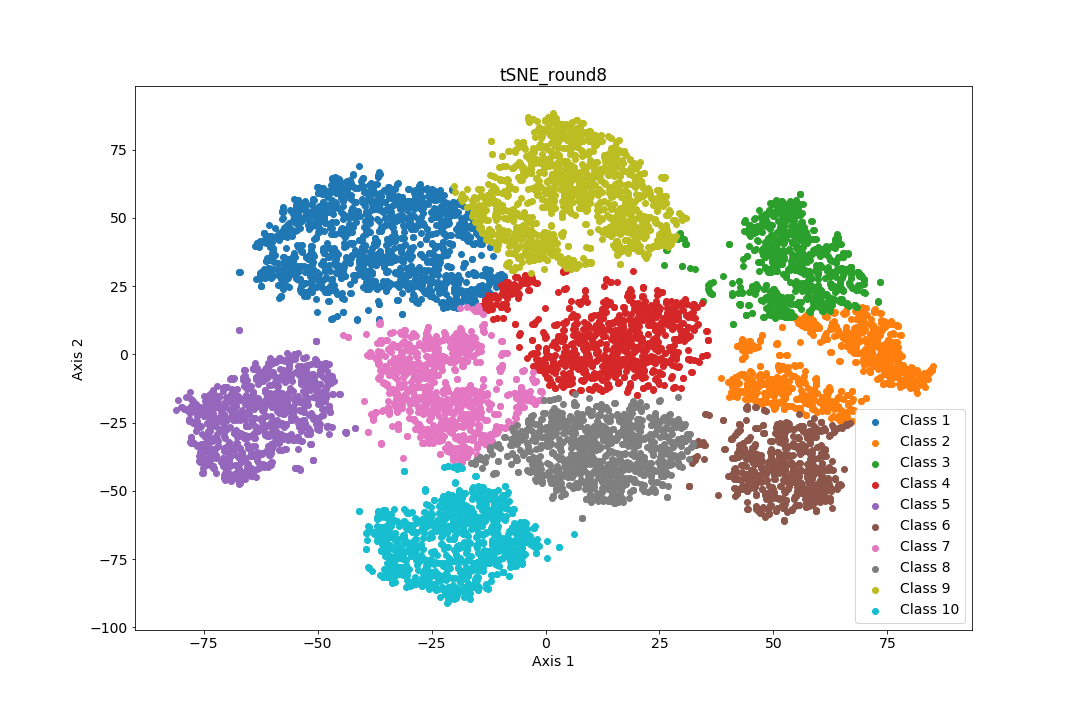
\includegraphics[width=1.1\linewidth]{tSNE_round8_kMeans.png}
		\caption{Clustering with tSNE: Round 8}
		\label{tSNE8}
	\end{subfigure}
\end{figure}

\begin{figure}[!htbp]
	\begin{subfigure}{.5\textwidth}
		\centering
		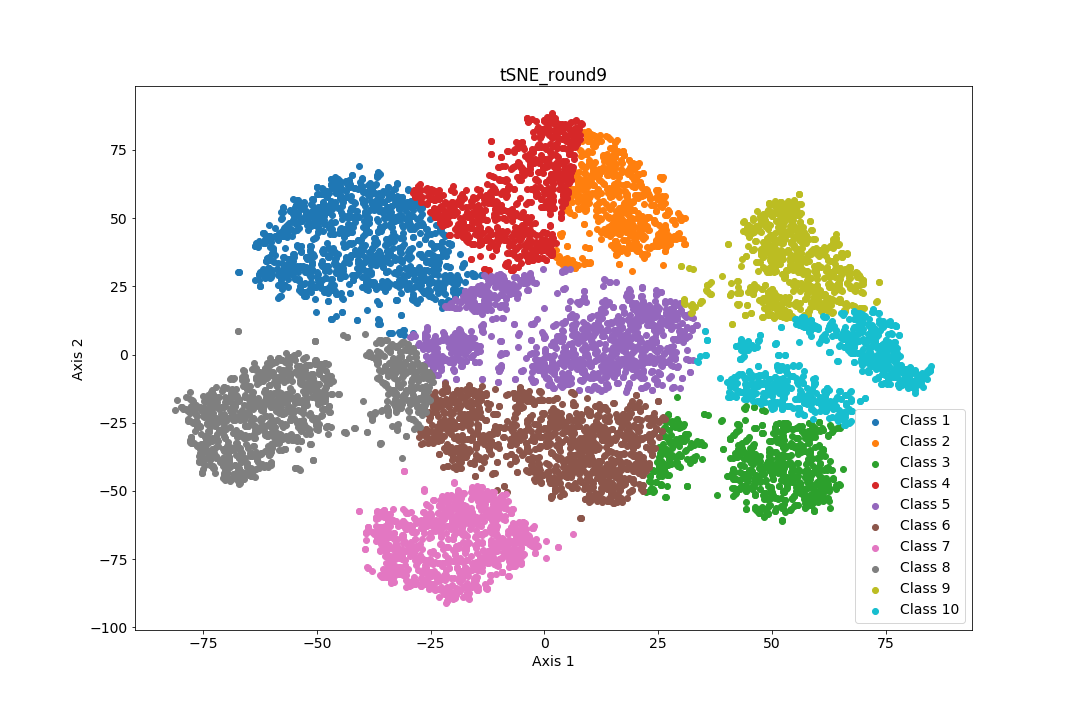
\includegraphics[width=1.1\linewidth]{tSNE_round9_kMeans.png}
		\caption{Clustering with tSNE: Round 9}
		\label{tSNE9}
	\end{subfigure}%
	\begin{subfigure}{.5\textwidth}
		\centering
		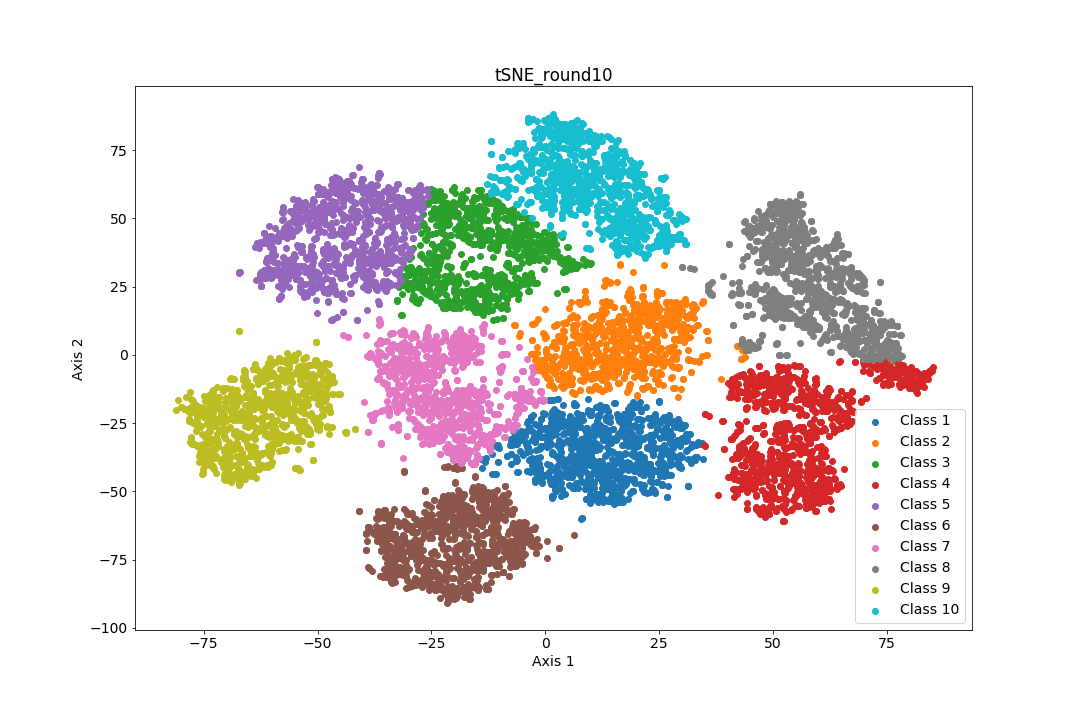
\includegraphics[width=1.1\linewidth]{tSNE_round10_kMeans.png}
		\caption{Clustering with tSNE: Round 10}
		\label{tSNE10}
	\end{subfigure}
\end{figure}


\end{mlsolution}


\end{document}
